\subsection{Flight Systems}
\subsubsection*{Airframe}
Given the aircrafts presented previously, the most suitable design for this project is the FireFLY6. However, even under expensive modifications, it may not be able to meet requirements \textbf{R4} and \textbf{R5}. An alternative was to purchase a hobby airframe, such as the Skywalker X8\cite{ref:x8} and design an aircraft to emulate the design of the FireFLY6.\\

The X8 can easily be used to replicate the FireFLY6's motor configuration, and has sbeen shown to be capable of up to 155km of flight\cite{ref:range}, which far exceeds the requirements for the UAV Challenge. In addition, the X8 is purpose designed to mount various sensors (such as a camera) to its frame. Appendix \ref{sec:scope} presents a detailed analysis of several design options, comparing the purchase of various FireFly6 models to several designs based on the X8.

\subsubsection*{Flight Control}
The addition of a flight controller to the aircraft permits autonomous flight capabilities, including way point planning and motor control. The most viable (and well supported) options are the PixHawk\cite{ref:pixhawk}, APM 2.6\cite{ref:ardupilot}, and PX4\cite{ref:px4}. In order to achieve reliable and safe autonomous flight the controller must be fast and have sufficient storage for additional firmware/software to extend its capabilities. A comparison of each option may be found in \cite{ref:controller_comparison}, showing that given its larger memory storage, faster processor, and additional capabilities such as in-built gyroscopes and accelerometers, the PixHawk is the best choice for this project.

\subsubsection*{Controller Development}
The PixHawk flight controller has several flight control systems readily available for many types of aircraft (including fixed-wing and VTOL), but as of yet has no control system designed for a hybrid aircraft. Fortunately, the PX4 firmware (on which the PixHawk is based) is Open Source\cite{ref:ardupilotgit}, with several resources available\cite{ref:firmware1,ref:firmware2} to allow hobbyists and developers to customize the behaviour of their aircraft.

\subsection{Proposed Design}
Based on the discussion above, the initial design for this project will use a PixHawk flight controller in a Skywalker X8 airframe, mounted with three motors in a tri-coptor configuration, as with the FireFLY6. The aircraft will also be fitted with a transition system, to rotate the front motors and enable the aircraft to fly in both VTOL and fixed-wing modes. Finally, the aircraft will be mounted with various sensors, including a camera and LiDAR, to provide sensing capabilities for planning, obstacle detection and autonomous flight.

\subsection{Hardware Architecture}
\red{Higher level stuff should go first.\\}
\red{Reference the design from the winning team last year, and the stuff they have that we still need (ie rocket m5)\\}
\red{Basically how we intend to meet every requirement for the challenge. Put in circuit diagrams here, archetecture, information regarding long range network transmitters, and basic intro to sensors, automation and transition. Basically introducing what the overall plan looks like and what we have covered from that. Maybe do a chart or table or something.}

Figure \ref{fig:hardwarearch} shows the hardware architecture that was planned for the current and future teams.

\begin{figure}[!h]
	\centering
	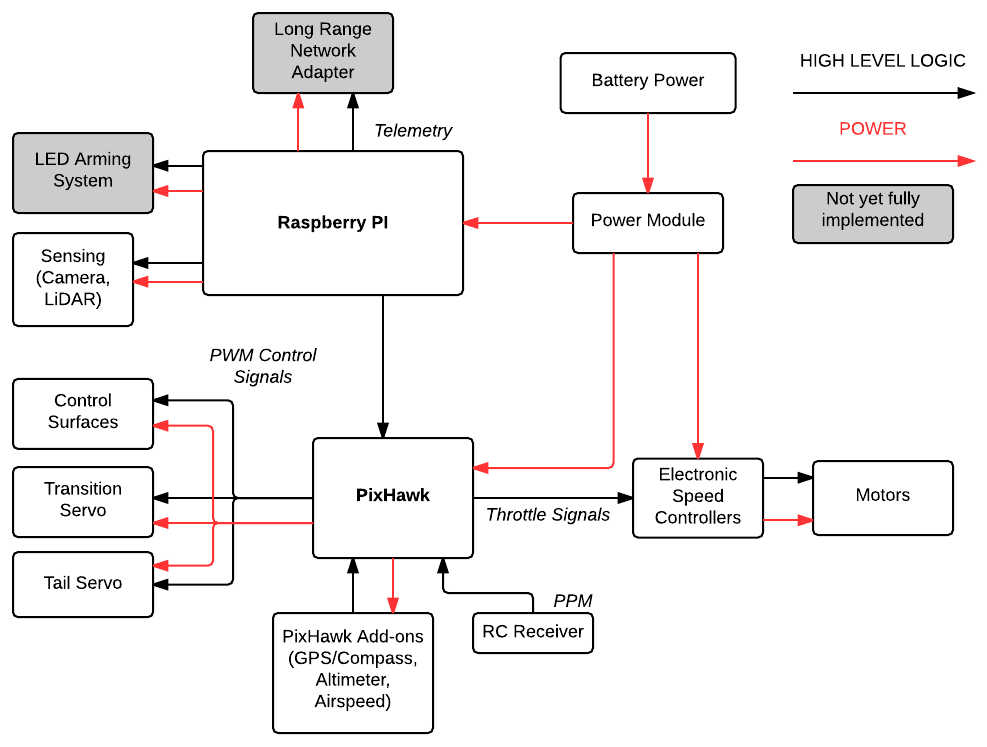
\includegraphics[width=400pt]{\IMAGEPATH /Diagrams/hardware}
	\caption{Architecture diagram for aircraft hardware}
	\label{fig:hardwarearch}
\end{figure}

\subsection{Basic Configuration}
The initial design of the aircraft was first modelled using eCalc\cite{ref:ecalc}, a commonly used web tool in the aircraft building community for calculating the performance of aerial vehicles. This site has a vast collection of empirical data for motors, propellers, batteries and aircraft configurations and boasts an accuracy of $\pm$10\% for all calculations. Examples of the modelling process can be found in Appendix \ref{sec:ecalc}. Figure \ref{fig:fixed} and Figure \ref{fig:vtol} show the final specifications for the configuration chosen on eCalc for the current prototype. Before any testing or calculation, this gives a good estimation of how well the aircraft will complete objectives. With an estimated 17.5 minutes of hover time and a climb rate of $9.9ms^{-1}$, this was determined to be significantly more than enough for the two take off and landing maneuvers required, leaving enough power for the fixed-wing flight in-between. Although eCalc gives a cruising speed of fixed wing flight, it does not give an estimation of maximum flight time while cruising (as power could be saved at level flight).

\subsubsection*{Layout}
To achieve the novel transition system sought after from the start of the project, the optimal motor configuration was investigated for the job. Having seen the capabilities of the FireFLY6 aircraft, a tri-coptor formation of the motors was selected.\\
		
A tri-coptor Y-3 configuration (three motors positioned in the shape of a `Y') was selected over a Y-6 (six motors), as it would lead to a lighter and cheaper aircraft. However, the aircraft was designed to be capable of being 'upgraded' to a Y-6 configuration if the need arose. The three motors would provide lift in VTOL mode, the front two motors being mounted vertically utilizing a mounting system capable of being rotated forwards $90^{\circ}$ to facilitate the transition system and fixed-wing flight. The rear motor mount system was designed to be tilted laterally through the use of a servo-motor to enable the yaw mechanism of the aircraft.

\subsubsection*{Airframe}
Through research, (see [ref]) the Skywalker X8 was chosen as a pre-designed `off the shelf' airframe. It offers a large amount of under canopy storage room, the greatest wingspan to weight ratio of the airframes investigated, fast low power cruise speeds, was stated to be capable of carrying a maximum all-up-weight (AUW) of greater than 3.5kg, was well priced, and available  from Australian suppliers. The fact that it is made out of EPO foam also made it easy to modify into the required hybrid frame. Design and development of critical subsystems started from here] 
\todomessage{reference lit review x8 choice?}
		
		
\subsubsection*{Carbon Fiber Poles and Supports}
The hybrid frame was created using a combination of two 12mm carbon fiber poles (front and back) and 3D printed mounts and supports. As gear systems, mounts and legs needed to be attached, all holes in the rod due to fastening were drilled parallel to the base of the aircraft in order to minimize any reductions in strength (as the top and bottom of the poles have tensile and compressive stresses when hovering).
	
\subsubsection*{Motor}
The motors chosen needed to efficiently hover, but at the same time be able to cruise in fixed wing mode using minimal battery power. As such, the Turnigy SK3 3542 800kv motors were chosen. They are efficient, well priced, well reviewed and very effective at completing both objectives. They were also the motors used by \red{[CITE VID]} to achieve long range flight.
	
\subsubsection*{Propellers}
Modelling using eCalc suggested that smaller propellers provide better performance in fixed wing flight (less weight and drag), but larger propellers are better suited for VTOL (more thrust), with modelling presented in \ref{sec:ecalc}. As such, two sets of propellers were purchased (11$\times$5.5 and 12$\times$6) in both plastic and carbon fiber.
\todomessage{elude to tests planned from the start}
	
\subsubsection*{Servo-motors}
Servo-motors were required to enable front transition system functionality and the back yaw system. Both servos chosen were Turnigy TGY-4409MDs, capable of 8.65kg.cm of torque at 5V, which was shown to be more than the required amount. 
		
\subsubsection*{Batteries}
The primary concern for maximizing flight time/range is by reducing weight. Multistar 8000 mAh batteries were selected as they allow for a much higher capacity at a lighter weight than conventional Lithium Polymer batteries. For flight testing the current prototype, two in parallel are being used. 
	
\subsubsection*{Flight Controller}
Following the discussion presented in \cite{ref:controller_comparison}, the PixHawk flight controller was found to be more powerful and faster, and more importantly, easier to reconfigure and add software to.

\subsection{3D Printing}
In order to enable proper stable and robust mounting of all motors and mounting systems, custom prototyping using 3D printed parts and iterative design was utilized to fit within the X8 frame. The major components of design were split up into the `Motor Mounts', the `Front  Mounting System' and the `Back Mounting System'. Minor systems and all iterations are shown in Appendix \ref{sec:print}.\\

The Motor Mounts were required to secure each motor to it's corresponding mounting pole. While the basic design was straight forward, a couple of design iterations were required in order to come up with a truly robust design. Cylindrical inserts (also 3D printed) were utilized in order to prevent the crushing of the carbon fiber rod in the event of over tightening the fasteners and a hose clamp was used to ensure that an equally distributed squeezing force was applied from the mount to the pole.\\

\begin{figure}[!ht]
	\centering
	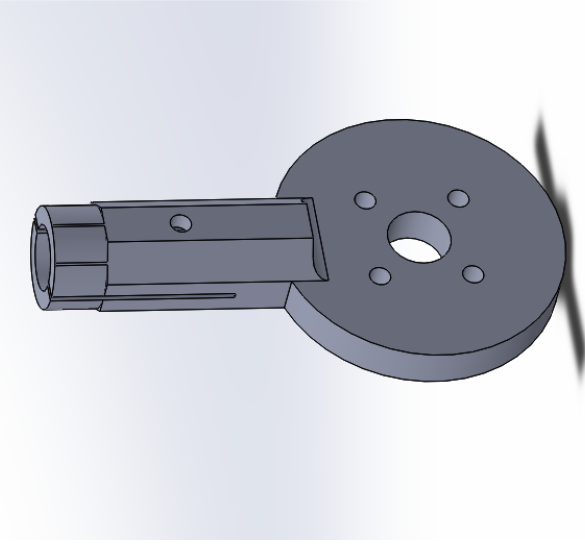
\includegraphics[width=160pt]{\IMAGEPATH Modelling/MotorMount3}
	\caption{Current iteration of the Motor Mount}
	\label{fig:designmotormount}
\end{figure}
	
The Front Mounting System was required to incorporate the transition system, while also being stable enough to withstand disturbances associated with being placed at the front of the aircraft. As such, it was designed to fit completely within the Skywalker X8's front recess, this was to ensure that the entire Front Mounting System was supported and that any lateral lode on the front mounting pole (i.e. incoming wind / still air) would be transferred through the entire aircraft and not just on the Front Mounting System itself.\\

\begin{figure}[!ht]
	\centering
	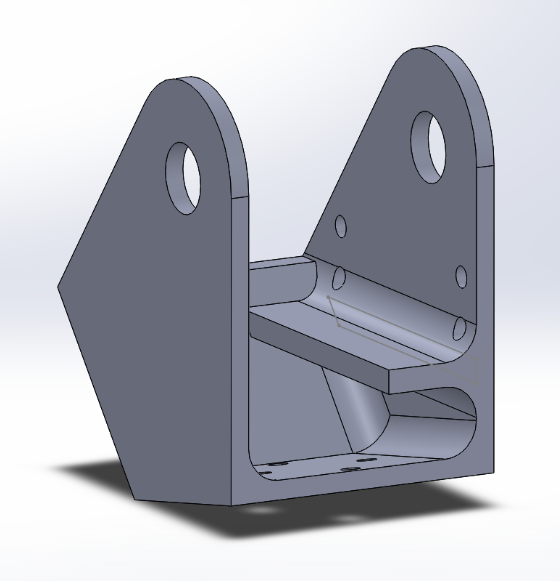
\includegraphics[width=160pt]{\IMAGEPATH Modelling/FrontMount3}
	\caption{Current iteration of the Front Mounting System}
	\label{fig:designfrontmount}
\end{figure}
	
The Back Mounting System was required to incorporate the yaw servo-motor system and also keep the back motor pole perpendicular to the front motor pole. A multi-webbed design was developed to keep the pole aligned in conjunction with the supplied Skywalker X8 tail ring support. Housing for the yaw servo-motor was built into the Back Mounting System to ensure a backlash-free mating between the gear and the pole.\\

\begin{figure}[!ht]
	\centering
	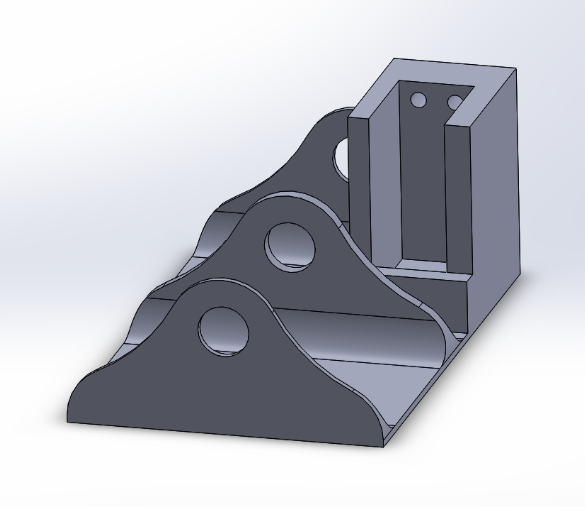
\includegraphics[width=160pt]{\IMAGEPATH Modelling/BackMount2}
	\caption{Current iteration of the Back Mounting System}
	\label{fig:designbackmount}
\end{figure}
		
The direction in which a design is 3D printed plays a vital role in where its strength and weaknesses lie. Each print was orientated to maximise the strength of the layers against the most likely mode of failure from the forces and moments being applied.\\

In order to achieve a ``true'' circle shape and thus lower friction for mated parts, critical ring shapes in designs were replaced by flatly printed ring inserts. These ring inserts were then either press fit into other printed components or ``merged'' onto other printed components using acetone. 


\subsection{Calibration}
\subsubsection*{Motor and Propeller Balancing}
To eliminate vibrations generated from propellers they were first balanced, which is accomplished by either adding mass (using tape, or similar) or removing mass (shaving off material) from either side of a propeller. As a non-destructive method was preferred, small pieces of tape were added to the propellers using the balancing apparatus shown in Figure \ref{fig:propbalancing} to ensure the mass distribution was equal.  Seismograph testing of the propellers before and after balancing showed a large decrease in vibrations.
\begin{figure}[!ht]
	\centering
	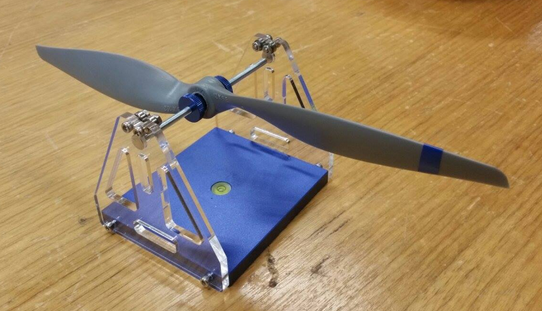
\includegraphics[width=300pt]{\IMAGEPATH /Prototype/prop_balancer}
	\caption{Propeller balancing apparatus, with propeller and tape to improve balance}
	\label{fig:propbalancing}
\end{figure}

\subsubsection*{Mass Balancing}
The center of gravity (CoG) of the new aircraft may be changed by repositioning the batteries (the heaviest items to be carried). The CoG needed to meet the following specifications:
	\\\\The center of mass had to be at the center of thrust of the VTOL. Due to the triangular nature of the propeller setup, this meantAs there are two propellers in the front and one in the back this would be one third of the distance from the front propellers to the back propeller (approximately 30cm from the front motors), resulting in an equal moment about the center of gravity. This would allow all motors to produce the same amount of thrust without causing the aircraft to tilt.
	\\\\The center of mass also had to be at the center of lift, which for Skywalker X8 is given as 44cm from the nose of the aircraft. The distance of the front motors from the nose of the aircraft is approximately 14cm. With the center of mass positioned 30cm from the front motors, the center mass and center of lift are coincident.
	
\subsubsection*{Electronic Speed Controllers Calibration}
The receiver and Pixhawk signals were calibrated into the electronic speed controllers (ESCs) by setting a minimum and maximum motor throttle. This was done by programming the ESCs simultaneously using the manufacturers manual.

\subsubsection*{Pixhawk Calibration}
The inbuilt compass and accelerometer of the Pixhawk required tuning each time the internal configuration of the aircraft changed in order to ensure level flight. This is achieved through performing specific calibration points in the open source program, Mission Planner. A once off power module voltage and radio calibration were also required, to ensure correct battery monitoring, and input. 
\todomessage{add more complexity of task, more paramaters}

\subsubsection*{PID Tuning}
The Pixhawk comes with in built PID parameters ready to be modified for all required control applications.  There are many ways to tune the Pixhawk PIDs. For the aircraft, basic tuning was first performed by setting the roll, pitch, and throttle gains and sensitivities to ensure stable and responsive flight controls. Then as recommended by the platform, an auto-tune was then completed and implimented on the craft to ensure the best possible PID values for the custom aircraft. This involved holding the aircraft in altitude hold mode while the aircraft tested responses and set the very best PID parameters. This was later verified by checking flight logs, for example Figure \ref{fig:tune1} shows untuned roll against to tuned roll for a disturbance . As shown in Figure \ref{fig:tune2}, when the wings were finally added the inertia, disturbances and weight of the aircraft changed significantly, and although there is more noise and overshoot, the original auto tune still kept stability. 

\begin{figure}[!ht]
	\centering
	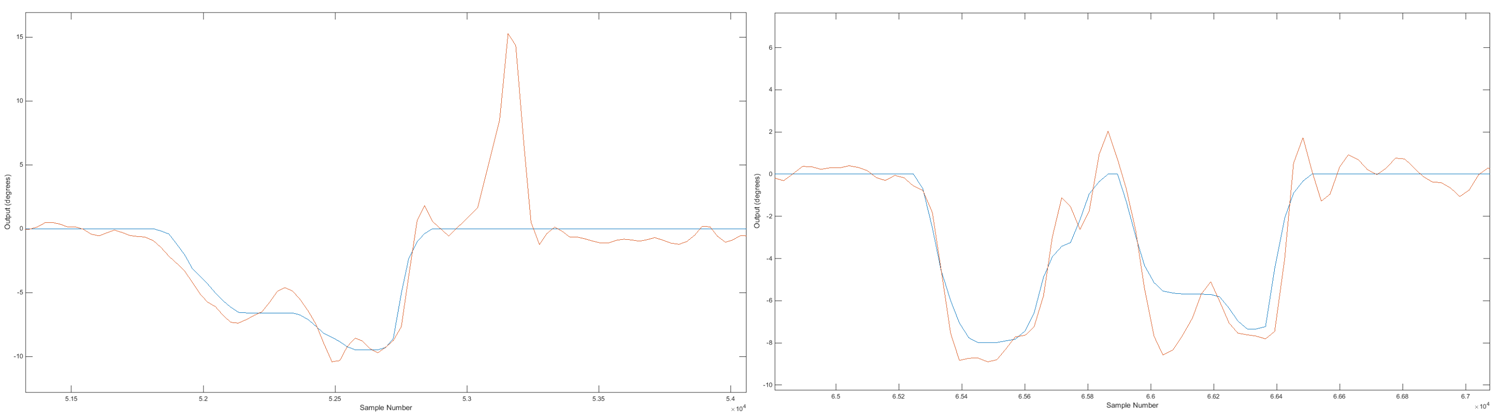
\includegraphics[width=500pt]{\IMAGEPATH /Data/tuned_untuned}
	\caption{Left: Untuned roll with significant overshoot. Right: Tuned roll.\\Blue = Desired, Red = Measured}
	\label{fig:tune1}
\end{figure}

\begin{figure}[!ht]
	\centering
	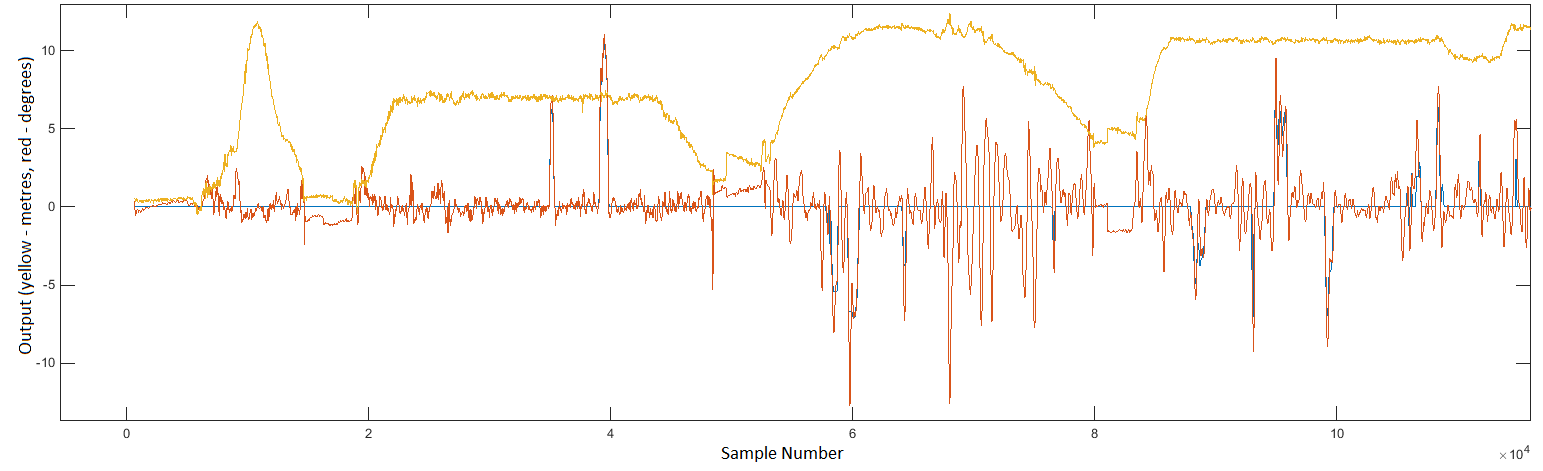
\includegraphics[width=500pt]{\IMAGEPATH /Data/tune_wings}
	\caption{Left half: Without wings. Right half: With wings.\\ Orange = Altitude}
	\label{fig:tune2}
\end{figure}


